In the manufacturing context, simulation refers to a ample spectrum of methodologies, techniques, and resulting software applications aimed at modeling and analyzing, through simulated experiments, the behavior of real production systems \cite{chung2003simulation, bangsow2010manufacturing}. 
The availability of models and tools to support the execution of accurate simulations of backbone processes in manufacturing is widely acknowledged as essential to making informed operational decisions at the shop floor level. 
Moreover, the high complexity of distributed value networks calls for reactive management systems that extend beyond the single company borders and disciplinary domains, envisioning the application of simulation tools at the core of novel cooperative digital environments. 

Historically, simulation solutions have been relegated only in the initial phases of factory design or in specific analyses targeting separated factory domains such as process validation, optimization of production layouts, scheduling and purchasing forecast~\cite{fowler2004grand}.
This limited scope stems from the fact that the application of simulation techniques to a traditional shop has proven to be a challenging and resource-eager activity, whereas the underlying models are often very sensitive to even small variations of context parameters resulting in time-increasing prediction errors. 
Consequently, the simulation has been regarded as some sort of chimera that promises great benefits and yet has never been really suitable for operative and reactive decisions. 

Nonetheless, the landscape is on the verge of a radical change thanks to the disruptive transformations witnessed in recent years and that are known by the term \textit{Industry 4.0} (I4.0)~\cite{Lu2017}. In particular, many players have adopted (or are in the process of adopting) approaches and methodologies typical of the Information and Communication Technology (ICT) industry with the aim of creating the factory of the future where the use of innovative technologies such as \textit{Machine Learning}, \textit{Big Data} and the \textit{Internet of Things}will be at the service of future production and managerial operations~\cite{Witkowski2017,Xu2014}.
In this context, the shop floor is redefined and envisioned as populated by self-monitoring fast-reconfigurable objects (mainly, machinery and robots), often referred to as \textit{Cyber-Physical Systems} (CPSs)~\cite{Jazdi2014}, equipped with computational resources and capable of establishing a capillary sensing of the shop floor by sharing their state information as well as coordination signals with other (even geographically distributed) stakeholders. 
Indeed, through different connection media (e.g., the RAMI 4.0 data buses~\cite{hankel2015reference}) this information can be exchanged, stored, and eventually used to finally achieve, among other things, reliable and accurate simulations in all phases of the factory life cycle. 
Moreover, since computational and reasoning capabilities are distributed with CPSs, 
the classical paradigm of simulation can be overturned by distributing the burden among the various CPS living in the Smart Factory~\cite{Lee2015,Hozdic2015} (i.e. gateways, production machinery, robots) exploiting emerging paradigms such as the \textit{Edge Computing}~\cite{georgakopoulos2016internet}. Such a scenario would have the undisputed advantage of increasing reactivity (because data movement is reduced) and simulation precision (each element could self-simulate using very accurate models because they are developed by the same machine manufacturers). 


Withal, thanks to the real-time and ubiquitous availability of information, the distance between the simulation run-time and the real factory situation results shortened. 
This enables the harnessing of digital avatars (a.k.a. \textit{Digital Twins}~\cite{Uhlemann2017}) to represent and interact with every actor involved in the manufacturing process; if a sufficient degree on composability is featured by such digital objects, even the whole shop floor can be mirrored in real-time within a simulation setup.   
The ability to mirror of real elements into their virtual representation, will enable the forthcoming platforms to simulate on top of constantly updated data, thus exploiting the full potentials of simulation; next generation solutions will, therefore, no more be relegated to the factory design and planning phases but exploited in the everyday work. In fact, if from one side the traditional approach based on \textit{what-if} scenarios, where the effect of (re-)design choices are analyzed without having to involve the real shop floor, will benefit from more accurate and fresh data, on the other hand this will provide support to \textit{now-what} decision-making processes, currently outside the boundaries of simulation, such as reactive reallocation of production resources to balance the production following an unexpected event or ensuing the on-time delivery of customer orders by reducing the effect of uncertainties.


Notwithstanding the staggering undertakings witnessed in these recent years, as pointed out in~\cite{pedrazzoli2014simulation}, there exist still relevant challenges affecting the maturity level in the adoption of I4.0 enablers in simulation and forecasting. 
Firstly, although high-performing computing services are available in the Cloud, simulation still under-exploits them, being almost always stuck in a centralized and localized vision that fails to take advantage of the opportunities offered by a distributed (Cloud) and, recently, on-board (Edge computing) paradigms.
Even the game-changing possibility to reliably collect and use in real-time data to mirror the factory is not currently exploited within simulation tools still struggling in the definition of virtual factory models~\cite{ciavotta2017microservice}.
Lack of flexible and extensible data models are hindering the emergence of multi-disciplinary simulation technologies to support the virtual investigation in a holistic perspective that promotes decision-making processes enriched by the analysis of the multiple domains interacting within the factory~\cite{hehenberger2016design}.
Ultimately, digital models need to evolve coherently with production systems along their life-cycles to leap over both punctual and paradigmatic transformations taking place in the shop floor and in the  information systems that support them \cite{azab2012simulation}.

This chapter aims at presenting and discussing some of the results obtained within FAR-EDGE, a European H2020 project, in the field of digital twin modelling and synchronization using data from the field with the purpose of improving simulation reliability. 
The rest of the chapter is structured as follows...




FAR-EDGE’s fundamental goal is to devise and develop an Edge computing solution for the virtualization of the factory automation pyramid, in order to support strategically production-related activities during all phases of the engineering and factory life cycle. This objective entails the definition and realization of several software layers serving three high-level functional domains namely, \textit{Automation}, \textit{Analytics}, and \textit{Simulation} (see Figure~\ref{fig:architecture}) to meet the global challenges of mass-customization and reshoring.

\begin{figure}
	\centering
	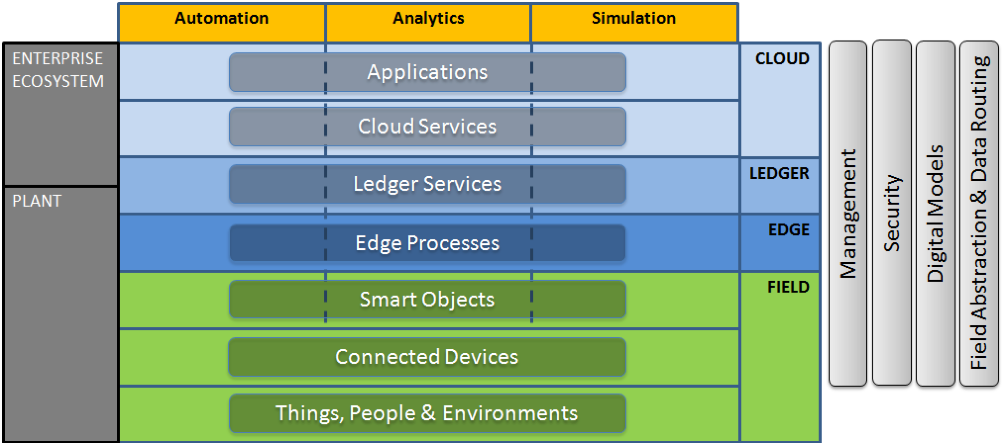
\includegraphics[width=\linewidth]{images/Far-edge.png}
	\caption{FAR-EDGE Reference Architecture overall view}
	\label{fig:architecture}
\end{figure}

As far as simulation is concerned FAR-EDGE aims at providing models and tools entailing functionalities for modeling CPS-based discrete manufacturing factories and simulating their behavior along the factory life cycle. 
In the FAR-EDGE vision, in fact, simulation is treated as a first-class citizen (as it is in Industrie 4.0 guidelines), being an enabler to implement layout and product optimization as well as to test what-if scenarios at minimal impact of regular shop activities. 
One of the main challenges of simulation in manufacturing is the so-called “Digital Continuity”. It consists in creating the conditions for a model to be up-to-date at any moment during the various phases of the life cycle of a factory. Thus, if from one hand this means that the interoperability of the model for virtualization and simulation must be maximized (engineering is by-nature a multidisciplinary process), from the other new mechanisms must be developed and put in place to allow the model to be in-synch with the shop floor evolving as automatically as possible with the state of the factory. As CPSs are subject to changes (e.g., for straining and aging), models should reflect those transformations. To detect this gap and update the model accordingly, raw data from the field (direct) or complex analysis algorithms (from Analytics domain) can be used. However, it is important to point out that the model itself must support model synchronization functionality natively in order to decouple the FAR-EDGE architecture, which must be independent of the particular factory, and the synchronization process that depends on the particular configuration of the factory at hand and ultimately on the model. 
For all the reasons presented above, the task of defining a suitable model is very ambitious; not only we aim at including in a single harmonic, coherent representation control, communication data collection and simulation data, but also at defining and being able to share a model describing the synchronization process.


